The written form of the Japanese Language is composed of three scripts, being two of them syllabic\footnote{In a syllabic script every character represents a complete phoneme which is not associated with any specific meaning. More precisely, those two scripts are considered to be moraic, a concept that is further explained in the Linguistic Appendix, at section \ref{mora}} and one of them ideographic.\footnote{every character of an ideographic script expresses a concept, rather than a sound} 
The syllabic scripts are both composed of 46 unique letters each and pose no big challenge to be learned, being thus studied in the primary school stage for native Japanese students. 
On the other hand, the ideographic script is composed of 2,136 official ideograms that are called the "Kanji" – more specifically "Jouyou Kanji" in the case of the official letters. 
These ideograms are the complete representation for the great majority of conceptual ideas in the Japanese language. 
As so, each Kanji carry a number of related meanings, some Japanese or "natural" readings, some Chinese or "radical" readings and finally some special readings to be used in the case of names.
Provided that a linguistic structure of such high complexity is part of the foundation of the Japanese written form, it becomes interesting to create efficient teaching tools to aid the learning process of the Japanese Kanji, a study that lasts to the end of high school to the native Japanese speakers themselves.

\section{Short History of the Japanese Writing System} \label{japhistory}
Although it is debated if the core base of the Japanese language is Korean or Altaic, it is accepted that the writing system of Japan was introduced from China. That is to say, prior to the introduction of writing from China, Japan did not have its own coherent writing System. This introduction came with the spread of Buddhism and is believed to have happened before the 5th century. The earliest found text dates from the early 8th century (the Kojiki). 

At first, the Japanese language was expressed solely through Chinese characters.
Several issues arose from this approach, since Japanese uses concepts of particles and conjugation that are different from Chinese, making it to require some few sounds repeatedly. At this stage of writing of Old Japanese (the Man'y\={o}gana writing system), Kanji were used both for semantic and phonetic functions. In the early 9th century, a writing system was invented by the Japanese to represent solely sounds. This type of script was called "Kana" and have two modern representatives, Hiragana and Katakana, which are further explained in Appendix \ref{hirakata}. Figure \ref{fig:kanji_to_hiragana} illustrates this adaptation of Kanji to pure syllabic graphemes in Hiragana.

\begin{figure}[h]
    \centering
    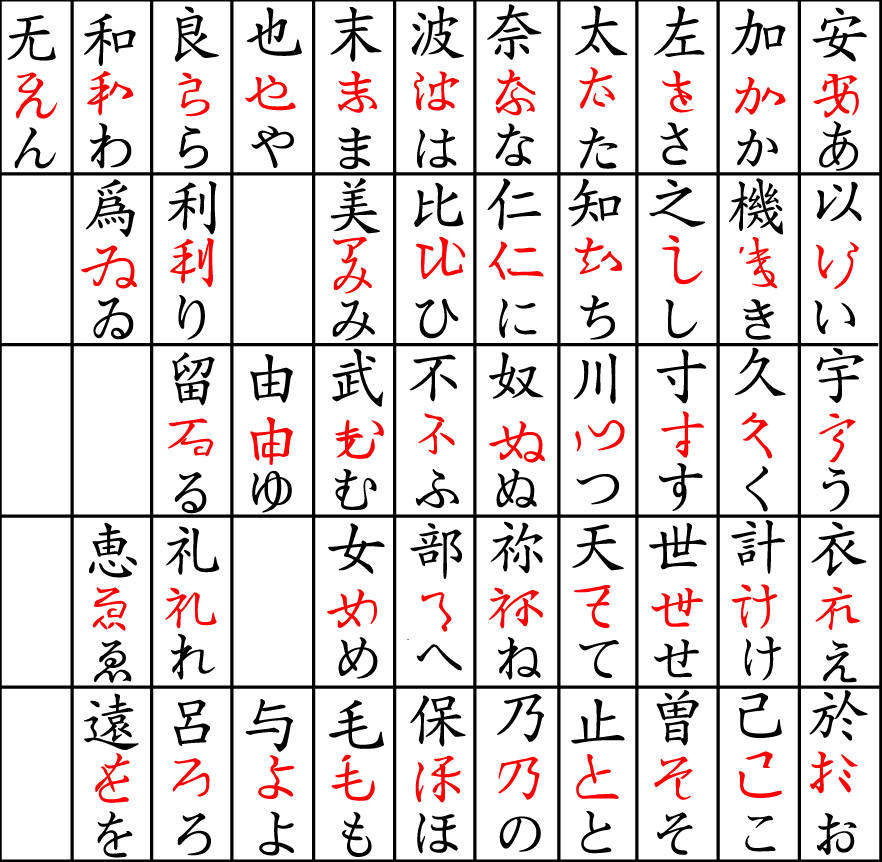
\includegraphics[width=0.8\textwidth]{Cap1/hiraganakanji}
    \caption{Adaptation from kanji to Hiragana, with the original Kanji at the top, an intermediary form in the middle and Hiragana at the bottom}
    \label{fig:kanji_to_hiragana}
\end{figure}

Prior to World War II, thousands of Kanji characters were in use in various writing systems and styles, leading to great difficulties to learning and teaching Japanese. To ease this problem, in 1946 the Japanese Ministry of Education created a list of the most commonly used 1,850 characters and declared them to be the official Kanji of the Japanese language. This list of official Kanji was called the T\={o}y\={o} Kanji (\jap{当用漢字}, literally "Chinese characters for general use"). This set of Kanji was proposed as an intermediary step for a plan that aimed at completely abolishing Kanji from the Japanese language, an ambitious plan that received strong opposition from the Japanese public.

In 1981 an updated list that added 95 additional Kanji to the T\={o}y\={o} Kanji was forwarded, and was named the J\={o}y\={o} Kanji, or Jouyou Kanji (\jap{常用漢字}, literally "Chinese characters for regular use"). In 2010 the official list was again reviewed, including additional 196 characters, while removing 5, forming the current Jouyou Kanji list with 2,136 official characters. Additionally, a second list of Kanji was created, the called Jinmeiy\={o} Kanji (\jap{人名用漢字}, literally "Chinese characters for use in personal names"). This second list supplements the Jouyou Kanji list, so that all proper names in Japanese should have all characters present in one of those two lists.

\section{Kanji Complexity Overview}\label{kanjicomplexity}

There are a number of factors that introduce complexity to the study of Japanese Kanji. Below, we list a a number of the most challenging issues.

\subsection{Various representations for the same Kanji}

For 212 Kanji in the J\={o}y\={o} Kanji there are two forms of the same character: the Old form (Ky\={u}jitai) and the Modern form (Shinjitai). Additionally, there are 4 characters listed in the Jouyou Kanji list that are not presented in Japan's basic character set, the JIS X 0208, and are thus commonly replaced by similar characters that are in this list. Therefore, in any proper statistical analysis it is required that both forms of these Kanji are mapped to the same concept. In Table \ref{tab:variants} we list 7 of these 216 variations.

\begin{table}[h]
\centering
\caption{Comparison of variants for 7 J\={o}y\={o} Kanji}
\label{tab:variants}
\begin{tabular}{|c|c|}
\hline
\textbf{\begin{tabular}[c]{@{}c@{}}New form/\\ Proper form\end{tabular}} & \textbf{\begin{tabular}[c]{@{}c@{}}Old form/\\ Adapted form\end{tabular}} \\
\hline
\Huge\jap{慎} & \Huge\jap{愼} \\ \hline
\Huge\jap{竜} & \Huge\jap{龍} \\ \hline
\Huge\jap{涼} & \Huge\jap{凉} \\ \hline
\Huge\jap{円} & \Huge\jap{圓} \\ \hline
\Huge\jap{尽} & \Huge\jap{盡} \\ \hline
\Huge\jap{礼} & \Huge\jap{禮} \\ \hline
\Huge\jap{頰} & \Huge\jap{頬} \\ \hline
\end{tabular}
\end{table}

\subsection{Multiple meanings associated to a single Kanji}
A further complication in the case of Japanese is that its roots are very apart from our own, so concepts we take as dissimilar in Romantic or Anglo-Saxonic languages may be considered to be related in Japanese, and therefore be grouped under the same ideogram. One such example is the ideogram \jap{気} that simultaneously means: spirit (as in soul), atmosphere (as in atmospheric pressure), mood/feeling, the mind and air.

\subsection{Multiple Chinese readings (on'yomi)}

As explained in Section \ref{japhistory}, the Japanese writing system was heavily influenced by Chinese. In this system, Chinese came to be the etymological root of compound words in Japanese. An analogy with the Anglo-phonic case would be the concept of Water, that can be worded as \textit{Hydro} (as in \textit{Hydraulics}) or \textit{Aqua} (as in \textit{Aquaphobia}). This kind of reading came to be known as the On'yomi. One situation that arose from this borrowing is that Chinese and Japanese use very different phonotactics. While in Japanese the only kind of different voicing is done by increasing the length of the voicing of a vowel (as in the proper name Tooru, or T\={o}ru), Chinese has five different kinds of intonations for the vowel parts of phonemes (for example: ma, m\={a}, m\`{a}, m\'{a} and m\v{a} are five different words in Chinese, differentiated solely through intonation), and also includes many consonant sounds that are not existent in Japanese. This incompatibility caused the Japanese mimics of the Chinese sound to be radically different than the original. Also, since the Chinese language entered in Japanese firstly through scholars and this was a process that lasted centuries, it occurred that miscopying was occasionally carried into Japanese as an accepted form or multiple steps of the phonetic evolution of the same word entered in Japan and multiple of those became accepted.

One such example of a Kanji with multiple on'yomi reading is \jap{数}, that represents the idea of figure or number. The officially recognized Chinese reading of this Kanji is "s\={u}", but four more readings are common: "su", "shu", "soku" and "saku". Note that the current reading in Chinese for this Ideogram is "sh\v{u}".

Figure \ref{fig:onyomihist} presents a histogram for the number of readings by Kanji. As it can be noted, most Kanji have only one Chinese reading, but about 470 have two readings and more than a hundred present three or more readings.

\begin{figure}[ht]
    \centering
    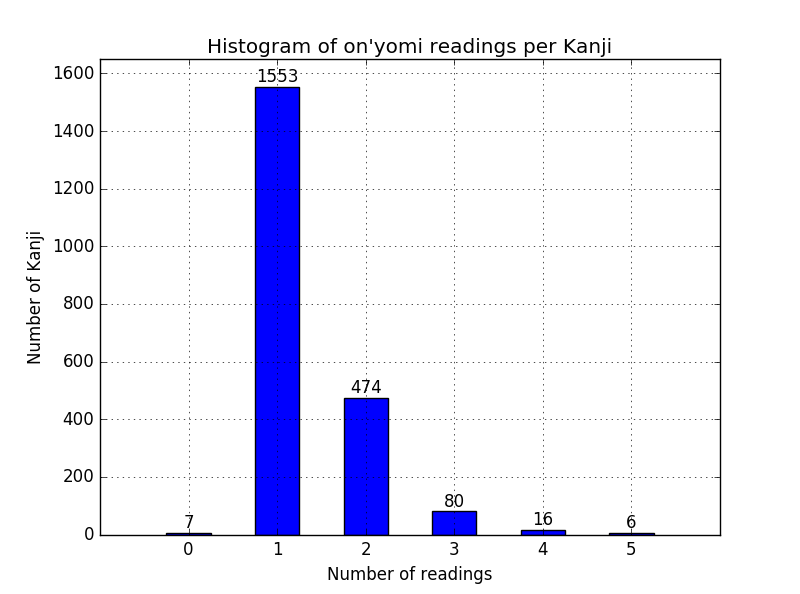
\includegraphics[width=\textwidth]{Cap1/HistogramOnYomi}
    \caption{A Histogram of the number of on'yomi readings by Kanji}
    \label{fig:onyomihist}
\end{figure}

\clearpage

\subsection{Multiple Japanese readings (kun'yomi)}

Even before the introduction of writing through Chinese influence, Japan already had a spoken language that had to be fitted to the imported characters. This kind of reading is mostly used for isolated Kanji, used as substantives, adjectives or verbs. To use again the analogy with Water/Hydro/Aqua, the kun'yomi reading would be the equivalent of the word "Water".

Once more, the Kanji \jap{数} is one that presents multiple readings. The officially recognized Japanese reading of this Kanjis are "kazu" and "kazo", though the readings "se", "wazurawa" and "shibashiba" are also used.

Figure \ref{fig:kunyomihist} presents a histogram for the number of readings by Kanji. As it can be noted, about half of the Jouyou Kanji have only one reading, but about 430 have two readings, 370 have no Japanese readings and almost 300 present three or more readings.

\begin{figure}[ht]
    \centering
    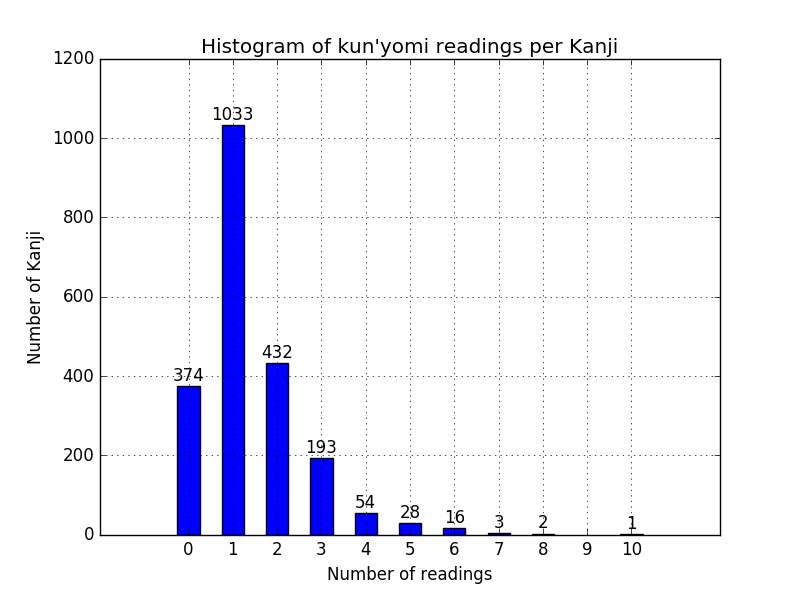
\includegraphics[width=\textwidth]{Cap1/HistogramKunYomi}
    \caption{A Histogram of the number of kun'yomi readings for Kanji}
    \label{fig:kunyomihist}
\end{figure}

\clearpage

\subsection{Readings for use in names (nanori)}

There is one more important type of reading for Kanji that should be considered by Japanese learners: the nanori reading. This type of reading represents readings for Kanji that are used in proper names (for example the name of cities, prefectures or people). 

The Kanji \jap{希}, which represents hope or request is a case with multiple nanori readings. This Kanji has the Chinese readings "ke" or "ki" and Japanese reading "mare", but in names it can be read as "nozo" or "nozomi" (note that "Nozomi" by itself is a full Japanese name).

Figure \ref{fig:nanorihist} presents a histogram for the number of readings by Kanji. As it can be noted, about 1200 Jouyou Kanji have no nanori readings, but 360 have one reading, 213 have two Japanese readings and about 350 present three or more readings.

\begin{figure}[ht]
    \centering
    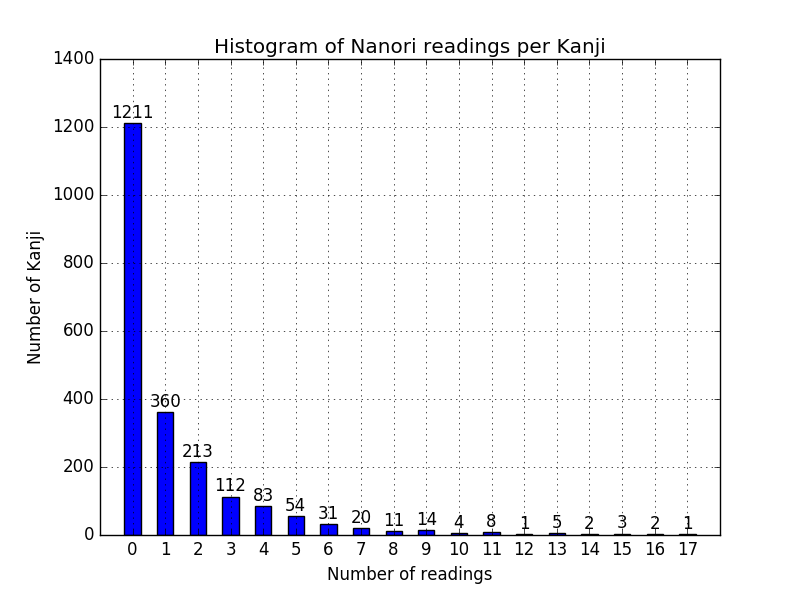
\includegraphics[width=\textwidth]{Cap1/HistogramNanori}
    \caption{A Histogram of the number of nanori readings for Kanji}
    \label{fig:nanorihist}
\end{figure}

\clearpage

\subsection{Irregular readings}

As if not enough, Kanji can also be read in a completely different fashion than its usual reading. One such example is the word \jap{一昨日} that can be read in a regular fashion as Issakujitsu (\jap{いっさくじつ}) where all parts of this word can be matched to its three ideograms: is/saku/jitsu. However, this word can also be read as Ototoi, a reading that have no connection whatsoever to the accepted Kanji readings of this word.

\subsection{Conclusion}

In brief, we can say that the task of teaching one single Kanji passes through teaching:
\begin{itemize}
    \item How this Kanji is written (including stroke order);
    \item One or more possibly dissimilar conceptual ideas to associate with it;
    \item Zero or more Chinese readings;
    \item Zero or more Japanese readings;
    \item Zero or more Naming readings;
    \item Possible words where it appear with an irregular reading;
\end{itemize}

\section{Present approaches for learning Kanji}\label{intro:presentapproaches}
A number of different methods have been proposed to teach the Japanese Kanji. For Japanese natives, the Japanese Ministry of Education have selected a list of 1,006 Kanji, the Ky\={o}iku Kanji (\jap{教育漢字}, literally the "Educational Kanji"). This list divides those 1,006 Kanji that are expected to be learnt by a native Japanese from grades one through six. Note that among Kanji of the same grade there's no order established by the Ministry of Education, and thus each school can choose the order according to its own preferences. The remaining 1,130 Kanji are expected to be studied through the three years of Junior High School. The number of Kanji that are selected for each grade is presented in Table \ref{tab:kyouiku}.

\begin{table}[ht]
\centering
\caption{Number of Kanji to be taught per grade}
\label{tab:kyouiku}
\begin{tabular}{|c|c|}
\hline
\textbf{Grade} & \textbf{Number of Kanji} \\ \hline
First & 80 \\ \hline
Second & 160 \\ \hline
Third & 200 \\ \hline
Fourth & 200 \\ \hline
Fifth & 185 \\ \hline
Sixth & 181 \\ \hline
\end{tabular}
\end{table}

This list of Kanji was developed through the combination of multiple different approaches, and do not directly reflect the frequency that these characters are present in Japanese media. Additionally, this list was put together with consideration to the age of the child in question. Considering that a First Grade child should be around 6 years old, the first grade Kanji refer to concepts that should be familiar to children that age, such as sun, moon, th ordinal numbers (1 through 10, 100 and 1,000), left, right, big, small, male and female. One example that shows how this list may not be the ideal for non-native speakers to follow is the Kanji \jap{関}, which means "to be related" or "connected". This Kanji is only taught in the fourth grade to Japanese students, but it is the 56th most common Kanji that is used in the Japanese version of Wikipedia.\footnote{This data is the result from a study made in this work, which can be found in chapter \ref{chap:frequency}.}

Another Source of order to study Japanese characters is the list that was provided by the JLPT – the Japanese Language Proficiency Test (\jap{日本語能力試験}). The organization responsible for this exam provided Kanji lists for each of its 4 levels of certificates: 103 Kanji for level four, 181 additional Kanji for level three, 739 additional for level two and finally 903 additional for level one, totalizing 1926 Kanji. Since its renewal in 2009, the JLPT became a five levels exam and stopped providing Kanji list. Since those official lists take in consideration non-native Japanese students, it is still a widely used guide to the order of Kanji to be learnt, although no order withing this levels was predetermined by the JLTP organization.

With this and other issues presented in section \ref{kanjicomplexity}, it is evident that non-native speakers can benefit much with learning media that are targeted specifically to their needs. Below are listed a number of different media that seeks to teach Japanese Kanji to non-native speakers, each followed by a critique of pros and cons.

\subsection{Learning Books}

\subsubsection{Kanji Look and Learn}

Kanji Look and Learn\cite{kanjilookandlearn} is a book by a collaboration of 5 Japanese teachers and is one of the most famous books for learning Japanese Kanji. In fact, it is a series of books that divides Kanji according to its grade on the previous lists issued by the JLPT organization. Figure \ref{fig:lookandlearn} presents the book cover and a small excerpt of the book.

\begin{figure}[ht]
    \begin{subfigure}{0.5\textwidth}
    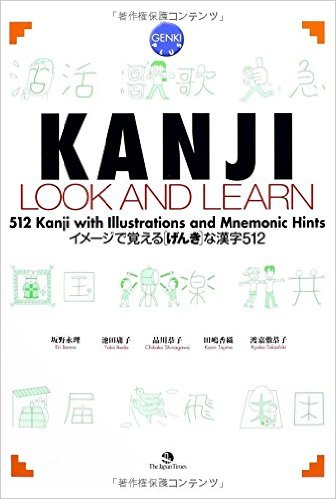
\includegraphics[width=0.9\linewidth]{Cap1/LookAndLearnKanji}
    \caption{Cover of Kanji Look and Learn.}
    \label{fig:lookandlearncover}
    \end{subfigure}
    \begin{subfigure}{0.5\textwidth}
    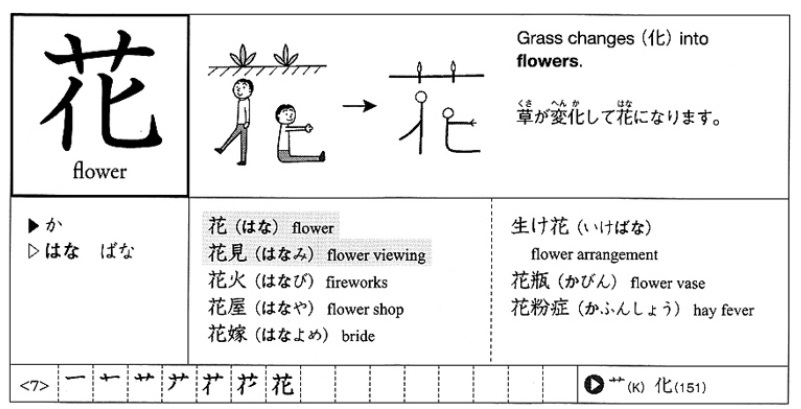
\includegraphics[width=0.9\linewidth]{Cap1/LookAndLearnPage}
    \caption{Excerpt from the book.}
    \label{fig:lookandlearnpage}
    \end{subfigure}
    \caption{Cover and Excerpt from Kanji Look and Learn.}
    \label{fig:lookandlearn}
\end{figure}

Like all the other examples of this section, this is a great book. Some advantages it has are:
\begin{itemize}
    \item Shows visual representations for Kanji using real life objects;
    \item Shows Japanese and Chinese readings;
    \item Presents multiple examples per Kanji;
    \item Displays stroke order;
    \item Separates Kanji among morphological radical parts;
    \item It has a simple clean interface for each Kanji;
\end{itemize}

Some limitations it faces are:
\begin{itemize}
    \item As any book, finding an information can be hard, encouraging a passive form of study (indexing problem);
    \item No Nanori readings are presented;
    \item Just a small number of Japanese and Chinese readings are presented;
    \item Even if radicals are broken up, it is hard to answer simple questions as "which other Kanji shares this same radical" or "is this Kanji visually similar to any other Kanji" or "is this Kanji a sub-component of any other Kanji";
    \item Definitions for words are short, making it possibly hard to understand the concept;
    \item Example words are not sorted by frequency, and a relatively small number of examples is shown;
\end{itemize}

\subsubsection{A guide to Remembering Japanese Kanji}

This Kanji study book by Kenneth G. Henshall\cite{henshall1988guide} is a classic and takes a very different approach to most other books. Firstly it develops from a serious and well structured history research that tries to uncover the true formation factors of the Kanji. It presents Kanji by the order established for grades in the Ky\={o}iku Kanji, and sorts Kanji alphabetically through their Chinese readings. Figure \ref{fig:henshallbook} presents the book cover and a small excerpt.

\begin{figure}[ht]
    \begin{subfigure}{0.5\textwidth}
    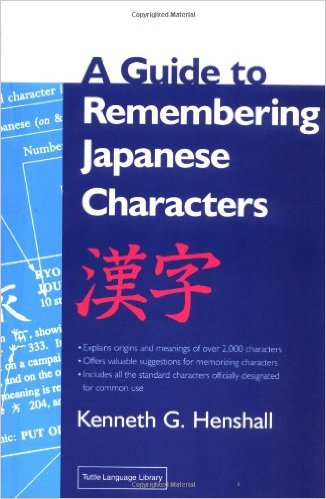
\includegraphics[width=0.9\linewidth]{Cap1/AGuideJapaneseCover}
    \caption{Cover of A Guide to Remembering Japanese Characters.}
    \label{fig:henshallbookcover}
    \end{subfigure}
    \begin{subfigure}{0.5\textwidth}
    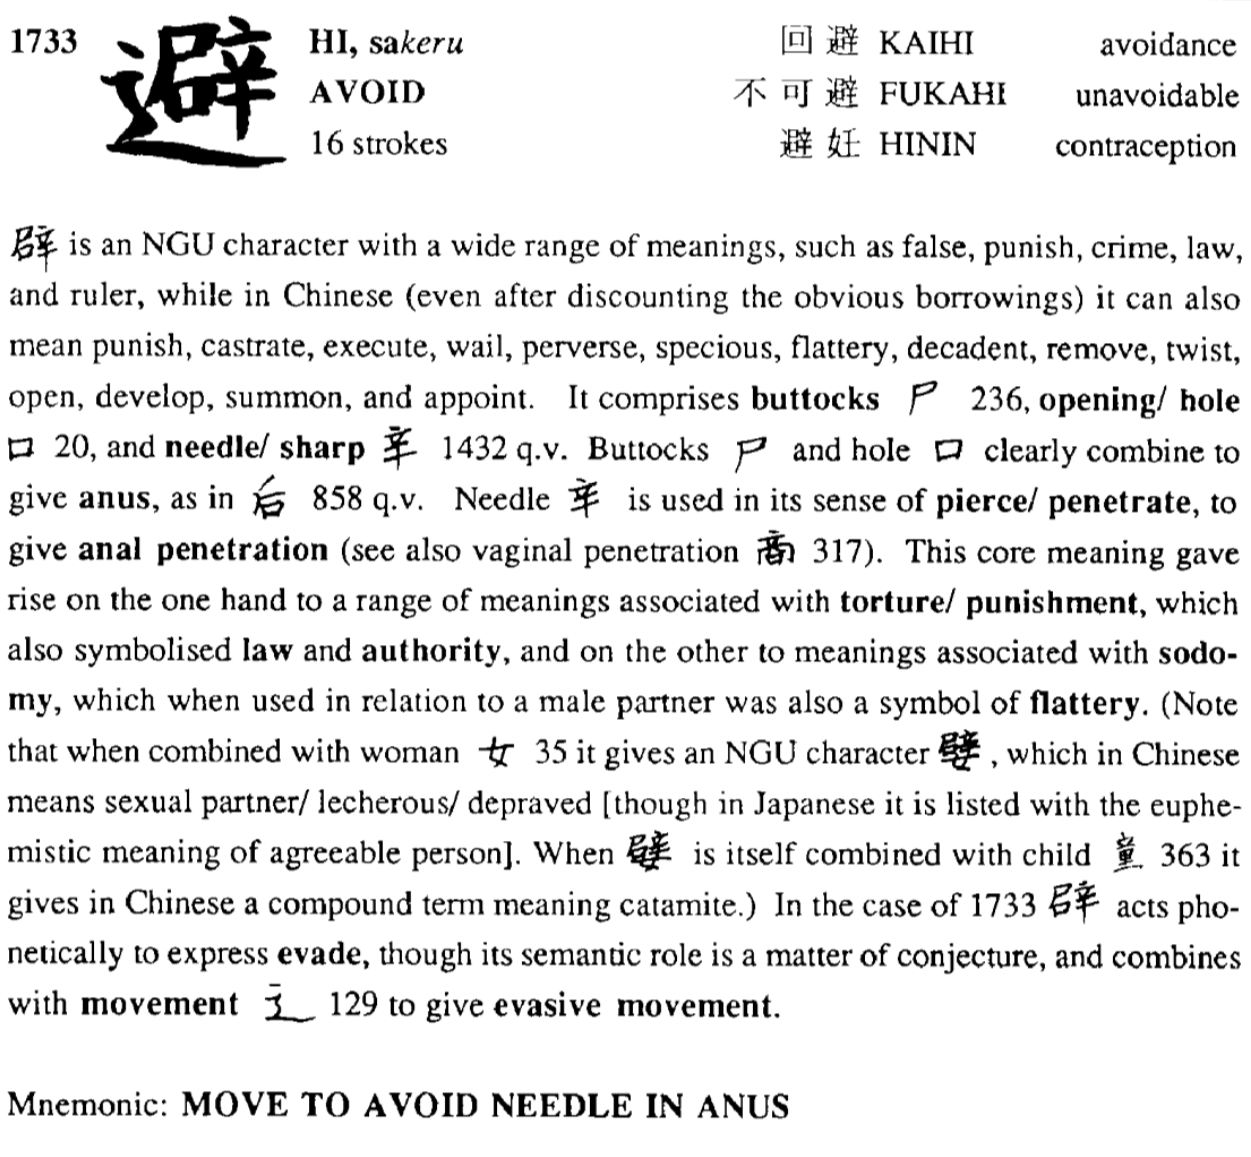
\includegraphics[width=0.9\linewidth]{Cap1/AGuideJapanese}
    \caption{Excerpt from the book.}
    \label{fig:henshallbookpage}
    \end{subfigure}
    \caption{Cover and Excerpt from A Guide to Remembering Japanese Characters.}
    \label{fig:henshallbook}
\end{figure}

Some advantages it has are:
\begin{itemize}
    \item Presents a very accurate description of the character morphological history, also defining which of its radicals are thought to have phonetic influence and which are thought to have conceptual influence;
    \item Shows On and Kun readings;
    \item Displays stroke number;
    \item Presents example words;
    \item Presents a mnemonic;
    \item Numbers Kanji in a fashion that is recognized by other important Japanese learning media, making it easy to refer to this book from ;
    \item cross references Kanji with other information that can be looked up through entry numbers;
\end{itemize}

Some limitations it faces are:
\begin{itemize}
    \item Once again, it presents indexing problems for looking up Kanji and relations between multiple Kanji;
    \item No Nanori readings are presented;
    \item Just a small number of Japanese and Chinese readings are presented;
    \item Does not always breaks a Kanji in its radical components;
    \item Definitions for words are short, making it possibly hard to understand the concept;
    \item Example words are not sorted by frequency, and a relatively small number of examples is shown;
    \item A great number of Kanji have very obscure history, provided that many of these have millennium of history, making this kind of study frustrating at times;
    \item Each entry presents a great deal of information which can not be minimized to browse only the essential pieces of information and connections;
\end{itemize}

\subsection{Websites}

\subsubsection{Jisho.org}

The Denshi Jisho project\cite{jishoorg} describes itself as: "Jisho is a powerful Japanese-English dictionary. It lets you find words, Kanji, example sentences and more quickly and easily". It is a free and open project that serves many functions, being in essence a very powerful and clean interactive dictionary in English for the Japanese language. As written in the website footnote, it was "lovingly crafted by Kim, Miwa and Andrew". Figure \ref{fig:jisho} presents an example entry of the Kanji dictionary functionality of this website.

\begin{figure}[ht]
    \centering
    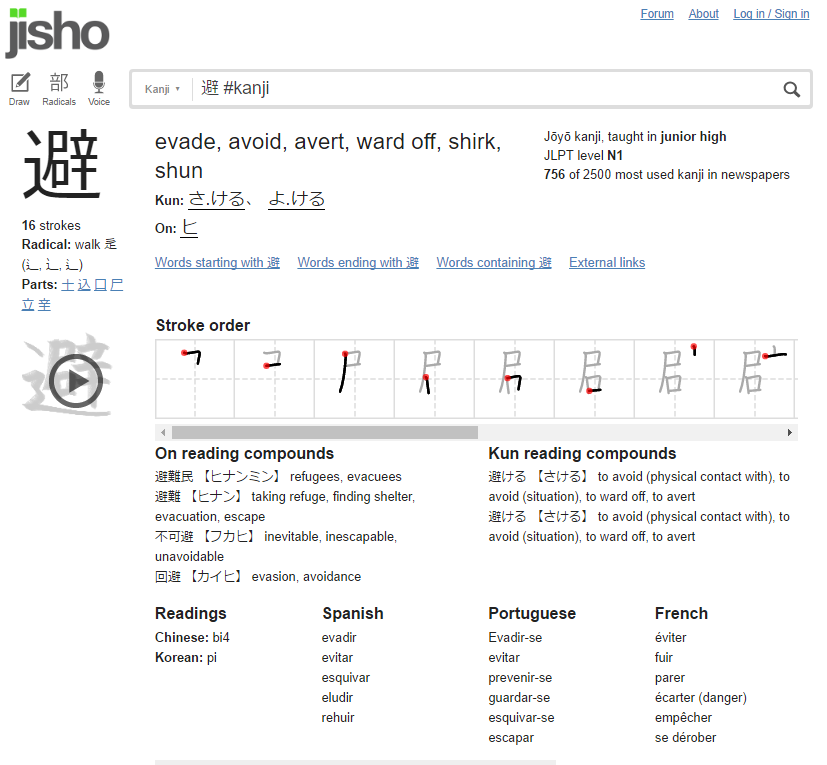
\includegraphics[width=0.8\textwidth]{Cap1/DenshiJisho}
    \caption{An example entry from Jisho.org}
    \label{fig:jisho}
\end{figure}

\begin{figure}[ht]
    \centering
    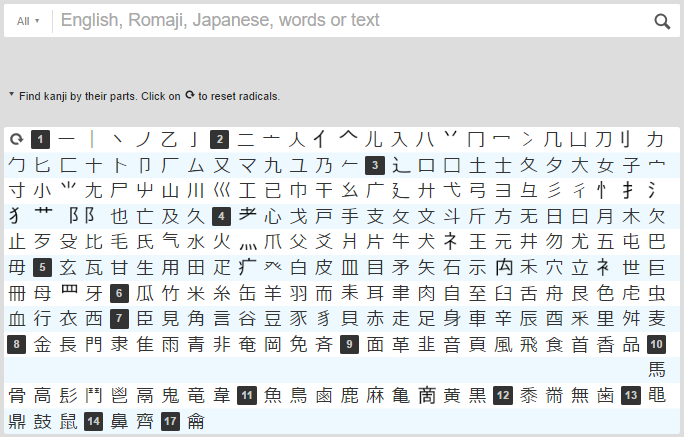
\includegraphics[width=0.5\textwidth]{Cap1/RadicalSearch}
    \caption{Radical look-up feature from jisho.org}
    \label{fig:jishoradsearch}
\end{figure}

It is a very useful website and has the following perceived advantages:
\begin{itemize}
    \item It has a very complete search capability, being able to look for Kanji from hand drawings, its radical parts (refer to figure \ref{fig:jishoradsearch}) and even through voice;
    \item Presents multiple links that can be followed for more information about a part, including some component parts;
    \item Provides a very complete set of definitions each Kanji can assume;
    \item Separates examples were it can be seen with its Chinese and Japanese Readings;
    \item Presents Nanori readings, when they exist;
    \item Displays definitions in multiple languages;
    \item Has animated and step by step stroke order guides;
    \item Displays information of frequency, JLPT level and Ky\={o}iku grade;
    \item It is free, which increases its reach;
\end{itemize}

Unfortunately, it has a few shortcomings:
\begin{itemize}
    \item The list of parts it is composed of is confusing, and does not follow any clear rule;
    \item Does not present simple relationships among characters, like which characters are composed of which other Kanji. For example, the Kanji in figure \ref{fig:jisho} is \jap{避} and has one big component that is not shown in Jisho's list: \chin{辟}. The provided list falls somewhat between trying to show all components to showing some that are apparently disconnected from this Kanji (such as \jap{込}). Following through the analysis of \chin{辟}, we note that it appears in four and four only J\={o}y\={o} Kanji: \jap{避}, \jap{璧}, \jap{壁}, \jap{癖}. This relationship cannot be attained in any easy way from Jisho's website, since the radical \chin{辟} is not one of its supported at its radical look-up screen (refer to figure \ref{fig:jishoradsearch}) either;
    \item Does not have a learning platform, only a browsing feature;
    \item Does not present a feature where characters are listed in ascending or descending order with their frequency;
\end{itemize}

\subsubsection{Wani-Kani}

Wani-Kani\cite{wanikani} is a paid web-app from where the "parts" and radicals used in Jisho.org were granted. It has a very complete learning feature, with a dedicated team to hand proof its data and designers to make elaborate custom mnemonic drawings. Its merits, according to its own description, are listed in figure \ref{fig:wanikani} and also explained below.

\begin{figure}[ht]
    \centering
    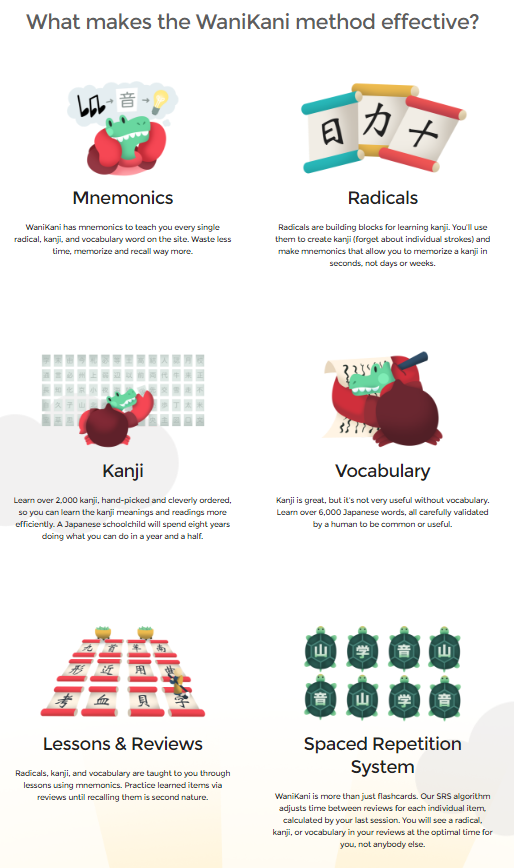
\includegraphics[width=0.8\textwidth]{Cap1/WaniKani}
    \caption{Wani-Kani advertised advantages}
    \label{fig:wanikani}
\end{figure}

\begin{itemize}
    \item Mnemonics: Has one mnemonic for every Kanji;
    \item Radicals: Approaches every Kanji from a building perspective, always teaching radicals prior to a Kanji;
    \item Kanji: Attempts to teach all 2,136 Jouyou Kanji, in a way that is "cleverly ordered";
    \item Vocabulary: It uses example words, as all previous books;
    \item Lessons \& Reviews: The website does not provide a browse feature (at least not until a character is considered to be learned), but only a Lessons and Reviews board;
    \item Spaced Repetition System: uses SRS theory\cite{baturay2009effects} to make spacing custom to each student;
\end{itemize}

Although all of these and other merits can rightfully be associated with Wani-Kani, it also has a number of perceived issues:

\begin{itemize}
    \item It is a paid service, which curbs its access rate and therefore its teaching potential;
    \item The website does not adapt well to its user preferences. For example: there is no functionality that lets the user edit and choose its own mnemonics in favor of those proposed unilaterally by Wani-Kani;
    \item Radicals are not well separated from Kanji, and the approach this website use to define which are the components of a Kanji (a process that is not always so straightforward) is not clear, sometimes referring to radicals for their visual appearance (As Kanji Look and Learn does) and some times for technical correctness (as Henshsall's Guide does);
    \item The "cleverly ordered" form does not follow any apparent technical guideline, just humans' subjective opinions;
    \item Shows a very limited number of words for each Kanji (a mean of three).
    \item Does not provide a leveling method, following the same bottom-up approach for every student;
    \item Its system does not facilitate browsing through Kanji, nor does it show important relations also missing from Jisho.org;
    \item Its Spaced Repetition System algorithm appears to treat Kanji as independent learning subjects, when in fact they have very rich relational structures among themselves;
\end{itemize}


\clearpage

\section{The need for a new way of learning}\label{intro:newway}

Taking in consideration all the advantages and disadvantages listed for the provided examples, we clearly notice that a new way of learning would greatly benefit Japanese learners. Firstly, this new way of learning should be a website, since it inherently holds many advantages in comparison with books, such as a bigger space for information, interactivity, indexing functions, browse and learning aids. 

On a second note, it can be noted that Jisho.org and Wani-Kani are already great learning aids, but each of them still holds some limitations. The work developed in this Academic Work is a stepping stone in the direction of creating a website that takes advantages of most of the functions that are considered to be advantages on those two platforms, as well as addressing their shortcomings.

Chapter \ref{chap:frequency} elaborates on the issue of taking Kanji frequency in Japanese media more seriously, so that the a student can have maximum success in learning frequent Kanji in minimal time.

% Chapter \ref{chap:readings} describes work in the direction of automatically matching Kanji readings to example words for a large number of those, also making associations of the Kanji to a Compiler Grammar.

Chapter \ref{chap:graphs} elaborates the concept of teaching order further, elaborating two graphs that relate Kanji among themselves (a morphological graph and a co-occurrence graph), as well as providing predictions of behaviors of students in analogy with random walk models with random restarts. 


Finally, Chapter \ref{chap:teaching} uses the knowledge obtained in previous chapters to propose specific details of the future website functionality in order to create an efficient teaching aid for the study of Japanese Kanji.